%% Copyright 1998 Pepe Kubon
%%
%% `two.tex' --- 2nd chapter for thes-full.tex, thes-short-tex from
%%               the `csthesis' bundle
%%
%% You are allowed to distribute this file together with all files
%% mentioned in READ.ME.
%%
%% You are not allowed to modify its contents.
%%

%%%%%%%%%%%%%%%%%%%%%%%%%%%%%%%%%%%%%%%%%%%%%%%%%
%
%     Chapter 3   
%
%%%%%%%%%%%%%%%%%%%%%%%%%%%%%%%%%%%%%%%%%%%%%%%%

\chapter{Problem Definition}
\label{ch:prob-def}

The traditional skyline query problem is to find the skyline points which are not dominated by any other points. In this thesis, we consider a variant of this problem. We consider a set of objects $S$ in an $n$-dimensional space and a query object $u$ in this space. The object $u$ may be a skyline point in some subspaces. We call these subspaces \emph{skyline subspaces}. The skyline subspaces query is to find out the \emph{skyline subspaces}. Different from the work of Tao et al.~\cite{tao2006subsky}: given a \emph{subspace} as a query, determine the sets skyline points in that subspace, the problem we want to solve is in a reverse way: given a query \emph{point}, determine the subspaces where the query point is in the subspace skyline. In this chapter, we will introduce the general skyline subspace queries and its applications in two different settings: skyline queries on graph and spatial skyline queries.

\section{General Skyline Subspace Queries}

\begin{definition}[Skyline]
For objects $u, v \in S$, $u$ dominates $v$ if and only if for all i, $(1 \leq i \leq n)$, $u.D_i \leq v.D_i$ and there exists a $j$ ($1 \leq j \leq n$) such that $u.D_j < v.D_j$. Object $u$ is a \emph{skyline object} if $u$ is not dominated by any other objects in $S$.
\end{definition}

\begin{definition}[Skyline Subspace]
Subspace $\mathcal{B}$ is a (non-trivial) $|\mathcal{B}|$-dimensional subspace of $\mathcal{D}$ 
if $\mathcal{B}\subseteq \mathcal{D} (\mathcal{B}\neq\emptyset)$.
For an object $u$ in space $\mathcal{D}$, 
the \emph{projection} of $u$ in subspace $\mathcal{B}$, denoted by $u_\mathcal{B}$
, is a $|\mathcal{B}|$-tuple$(u.D_{i_1},\dots,u.D_{i_{|\mathcal{B}|}})$,
where $D_{i_1},\dots,D_{i_{|\mathcal{B}|}} \in \mathcal{B}$, $u.D_i$ is the value of $u$ on $D_i$. If $u_\mathcal{B}$ is not dominated by any $w_\mathcal{B}$ in subspace $\mathcal{B}$ where $w \in S$, then $\mathcal{B}$ is a \emph{skyline subspace} for $u_\mathcal{B}$.
\end{definition}

\begin{definition}[Minimal Skyline Subspace]
A \emph{skyline subspace} $\mathcal{B}$ is a \emph{minimal skyline subspace} for object $u$ if and only if there is no such a \emph{skyline subspace} $\mathcal{C}$ for object $u$ that $\mathcal{C} \subset \mathcal{B}$.
\end{definition}

\begin{definition}[Skyline Subspace Queries]
Given a set of objects $S$ in an $n$-dimensional space $\mathcal{D} = (D_1,\dots,D_n)$ and a query object $u = (u.D_1,\dots,u.D_n)$ in space $\mathcal{D} = (D_1,\dots,D_n)$. The skyline subspaces query is to find all the \emph{minimal skyline subspaces} for query object $u$.
\end{definition}

\begin{table}[h]
    \centering
    \begin{tabular}{|l|l|l|l|}
    \hline
    points & $A$ & $B$ & $C$ \\ \hline
    $x$      & 4 & 2 & 3 \\ \hline
    $y$      & 3 & 3 & 3 \\ \hline
    $z$      & 2 & 4 & 1 \\ \hline
    \end{tabular}
    \caption{\label{tab:objects_example} A set of objects as our running example}
\end{table}

In Table~\ref{tab:objects_example}, if the query point is $y$, the minimal skyline subspaces of $y$ are $(A, B)$ and $(B, C)$. In subspace $(A, B)$, $x_{(A, B)} = (4, 2), y_{(A, B)} = (3, 3), z_{(A, B)} = (2, 4)$ and $y_{(A, B)}$ is not dominated by $x_{(A, B)}$ or $z_{(A, B)}$. 
In subspace $(B, C)$, $x_{(B, C)} = (2, 3), y_{(B, C)} = (3, 3), z_{(B, C)} = (4, 1)$ and $y_{(B, C)}$ is not dominated by $x_{(B, C)}$ or $z_{(B, C)}$. Therefore, $(A, B)$ and $(B, C)$ are both skyline subspaces. 
In subspace $(A, C)$, $y_{(A, C)} = (3, 3), z_{(A, C)} = (2, 1)$ and $y_{(A, C)}$ is dominated by $z_{(A, C)}$. There $(A, C)$ is not a skyline subspace. 
$(A, B, C)$ is a skyline subspace but it not a minimal skyline subspace because it is a proper superset of one of the skyline subspace $(A, B)$.

\section{Skyline Subspace Queries on Graph}
In this section, we introduce the skyline subspace queries on the graph setting. First, we will introduce a kind of graph such that each vertex in the graph contains several labels, denoted by a \emph{label graph}. We are interested in the distance between each vertex and each label. The set of distances between a vertex and all labels is represented by the \emph{label distance vector} of that vertex. The following shows the definitions of \emph{label graph} and \emph{label distance vector}.

\begin{definition}[Label Graph]
A label graph is defined as a undirected and unweighted graph $G = (V, E, L)$, with each vertex $v \in V$ contains a set of labels $L_v \subseteq \mathcal{L}$. $\mathcal{L}$ is the universal set of labels.
\end{definition}

\begin{definition}[Label Distance Vector on Graph in $d$-hop]
Given a label graph $G$ and a hop number $d$, Label Distance Vector of a vertex $v$ is $LV_v=\left\{\left(l_i, dist_i\right)\right\}$, $i = 1 \ldots n$. $l_i$ is a reachable label from $v$. $dist_i$ is the distance from vertex $v$ to the closest vertex that contains label $l_i$. If a label $l_j$ is not reachable by a vertex $u$ in $d$ hops, then $dist_j = \infty$
\end{definition}

\begin{definition}[Skyline Subspace Queries on Graph]
Given a label graph $G = (V, E, L)$, a query vertex $q$ and a number $H$, the skyline subspaces query on graph is to find all the \emph{minimal skyline subspaces} of $q$ in terms of the label distance vectors on graph.
\end{definition}

\begin{table}[h]
    \centering
    \begin{tabular}{|l|l|}
    \hline
    Skills         & Experts \\ \hline
    Accounting     & $u$     \\ \hline
    Bioinformatics & $y, w$  \\ \hline
    C++            & $w$     \\ \hline
    \end{tabular}
    \caption{\label{tab:skill_sets}An example of skill sets on LinkedIn profile}
\end{table}
    
\begin{figure}[h]
    \centering
    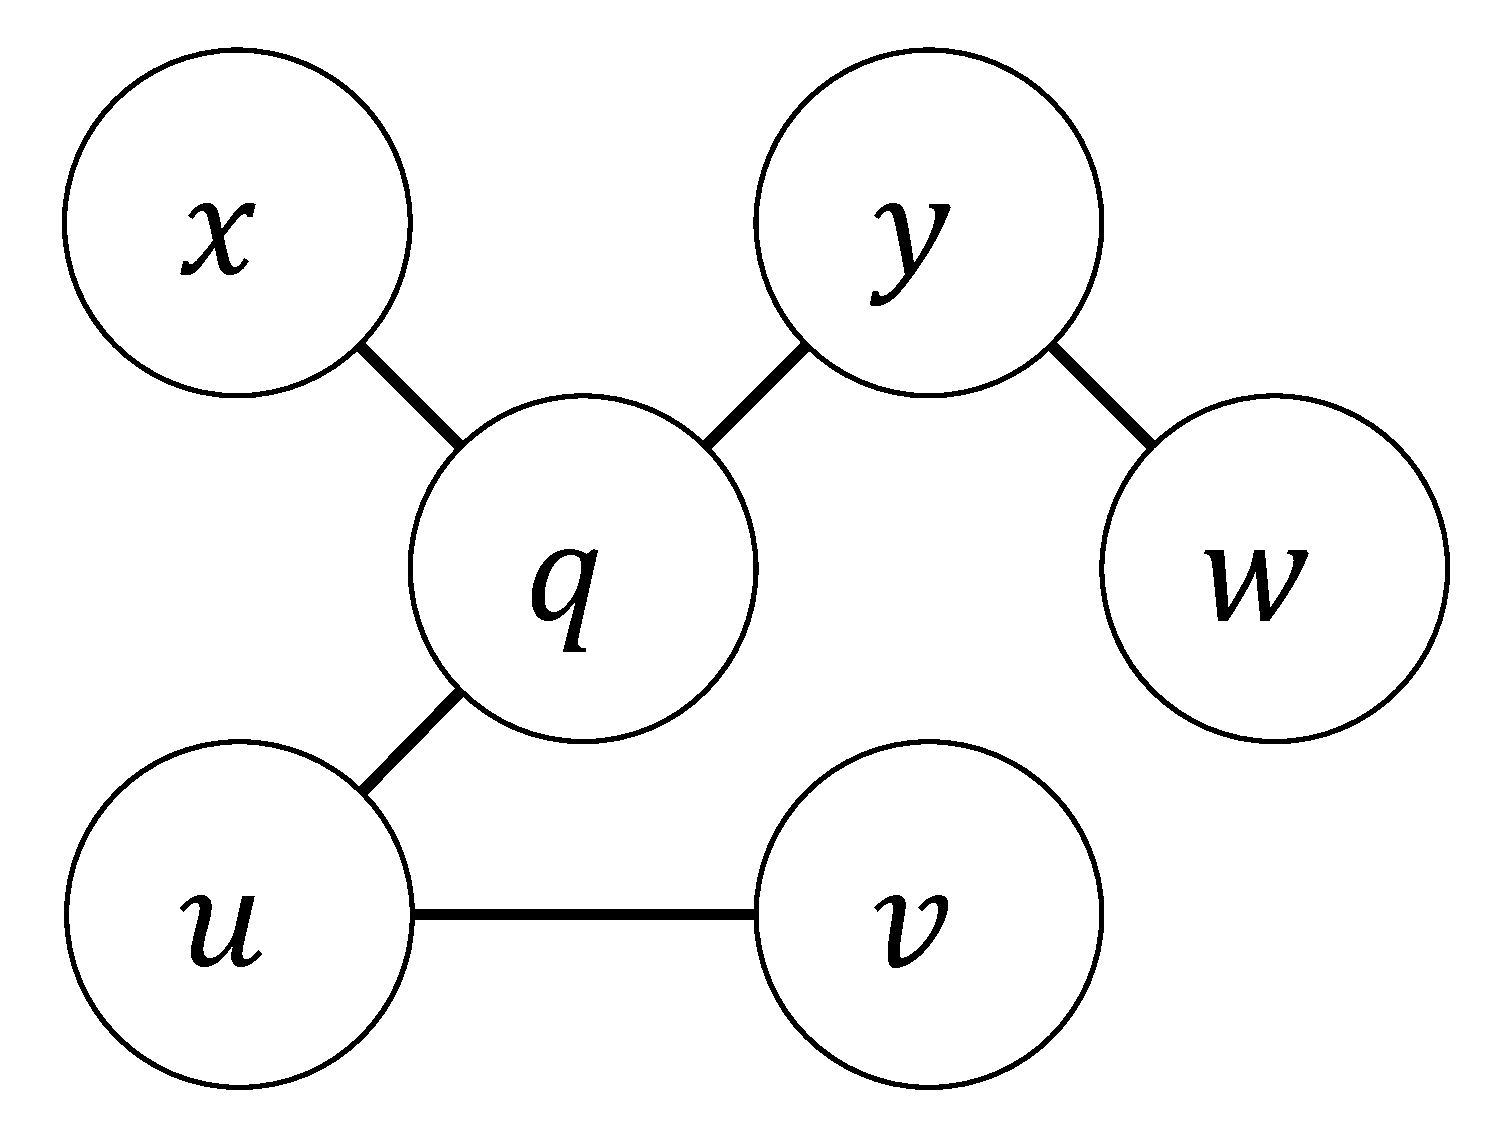
\includegraphics[width=0.3\textwidth]{figs/graph_example}
    \caption{An example of LinkedIn network}
    \label{fig:graph}
\end{figure}

Consider an example on LinkedIn to illustrate the skyline subspace queries on graph. In Figure~\ref{fig:graph}, a graph is represented by the LinkedIn connection network. Table~\ref{tab:skill_sets} shows the skills of each person of the LinkedIn network which can be treated as vertices with labels. 
Both of them together represent a \emph{label graph}. In Table~\ref{tab:skill_sets}, it shows that vertex $u$ has a skill of Accounting, vertex $w$ has skills of Bioinformatics and C++ and vertex $y$ has a skill of Bioinformatics. In this example, we want to compute the subspace skyline queries in $3$ hops.

\begin{table}[h]
    \centering
    \begin{tabular}{llll}
    \hline
        Distances & A & B & C \\ \hline
        $u$       & 0 & 2 & 3 \\ \hline
        $v$       & 1 & 3 & $\infty$ \\ \hline
        $w$       & 3 & 0 & 0 \\ \hline
        $x$       & 2 & 2 & 3 \\ \hline
        $y$       & 2 & 0 & 1 \\ \hline
        $z$       & 1 & 1 & 2 \\ \hline
    \end{tabular}
    \caption{\label{tab:distances_graph} distances between each person and each skill}
    
\end{table}

In the header row of Table~\ref{tab:distances_graph}, $A$, $B$ and $C$ stand for Accounting, Bioforinformatics and C++ respectively. The table shows the distances between each person and each skill. For example, the distance between $v$ and skill $B$ is $3$ because $y$ is the closest vertex to $v$ that contains label $B$ and the distance between $v$ and $y$ is $3$. Since C++ is not reachable by $v$ in $3$ hops, the distance between $v$ and $C$ is $\infty$. Each row of Table~\ref{tab:distances_graph} represents a \emph{label vector} of a vertex.
In this example, if the query point is $z$, the minimal skyline subspaces of $z$ are $(A, B)$ and $(A, C)$ because there is no such a vertex $w \in S$ that $w_{(A,B)}$ dominates $z_{(A,B)}$ or $w_{(A,C)}$ dominates $z_{(A,C)}$.


\section{Spatial Skyline Subspace Queries}

In this section, we will introduce spatial skyline subspace queries. Given a set of points in $2$-dimensional space. Some of the points will contain some labels. The distance between a point and a label is the Euclidean distance between that point and the closest point with that label. Our goal is to compute the skyline subspace queries on this spatial setting.

\begin{definition}[Spatial Label Distance Vector]
Given a set of points $P$, the Label Distance Vector of a point $v$ is $LV_v=\left\{\left(l_i, dist_i\right)\right\}$, $i = 1 \ldots n$. $l_i$ is a reachable label from $v$. $dist_i$ is the Euclidean distance from vertex $v$ to the closest vertex that contains label $l_i$.
\end{definition}

\begin{definition}[Spatial Skyline Subspace Queries]
Given a set of points $P$ and a query point $q$, the skyline subspaces query on Euclidean space is to find all the \emph{minimal skyline subspaces} in terms of the spatial label distance vectors.
\end{definition}

\begin{table}[h]
    \centering
    \begin{tabular}{|l|l|}
    \hline
    Categories     & Spots \\ \hline
    Asian Food     & $u$     \\ \hline
    Breakfast      & $y, w$  \\ \hline
    Cafes          & $w$     \\ \hline
    \end{tabular}
    \caption{An example of spots with categories}
    \label{tab:spot_category} 
\end{table}


\begin{figure}[h]
    \centering
    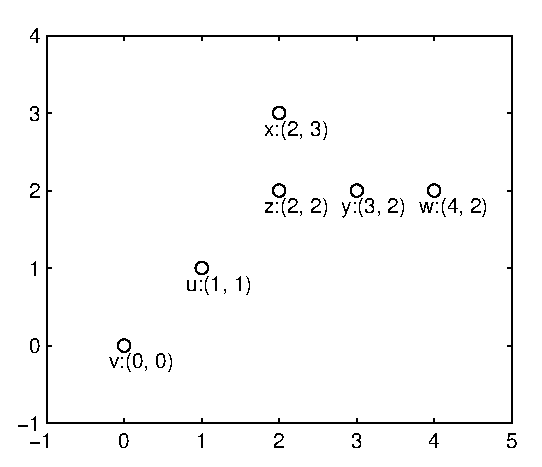
\includegraphics[width=0.5\textwidth]{figs/spatial_figure}
    \caption{An example of spatial locations of spots}
    \label{fig:spatial_map}
\end{figure}

Table~\ref{tab:spot_category} shows different spots with different categories. Figure~\ref{fig:spatial_map} shows the geometric locations of all spots. We consider each spot as a point in a $2$-dimensional space and the categories the spot contains as its labels.

\begin{table}[h]
    \centering
    \begin{tabular}{llll}
    \hline
    Distances & A & B & C \\ \hline
    $u$       & 0 & $\sqrt{5}$ & $\sqrt{10}$ \\ \hline
    $v$       & $\sqrt{2}$ & $\sqrt{13}$ & $\sqrt{18}$ \\ \hline
    $w$       & $\sqrt{10}$ & 0 & 0 \\ \hline
    $x$       & $\sqrt{5}$ & $\sqrt{2}$ & $\sqrt{5}$ \\ \hline
    $y$       & $\sqrt{5}$ & 0 & 1 \\ \hline
    $z$       & $\sqrt{2}$ & 1 & 2 \\ \hline
    \end{tabular}
    \caption{\label{tab:distances_spatial} Distances between each spot and each categories}
\end{table}

In the header row of Table~\ref{tab:distances_spatial}, $A$, $B$ and $C$ stand for Asian Food, Breakfast and Cafes respectively. The table shows the distances between each spot and each categories. In this example, if $z$ is the query point, then the minimal skyline subspaces are $(A, B)$ and $(A, C)$.


